\documentclass[border=10pt]{standalone}
\usepackage{tikz}
\usepackage{amsmath,amssymb}
\usepackage{xcolor}
\usetikzlibrary{arrows.meta,positioning,fit,calc,backgrounds}

\definecolor{riskpurple}{HTML}{e1cfe5}
\definecolor{infoblue}{HTML}{cce0f0}
\definecolor{stratorange}{HTML}{f8d7a9}
\definecolor{aggred}{HTML}{f4c4bb}
\definecolor{eqgreen}{HTML}{cce6cc}
\definecolor{gamegray}{HTML}{f4f4f4}

\begin{document}

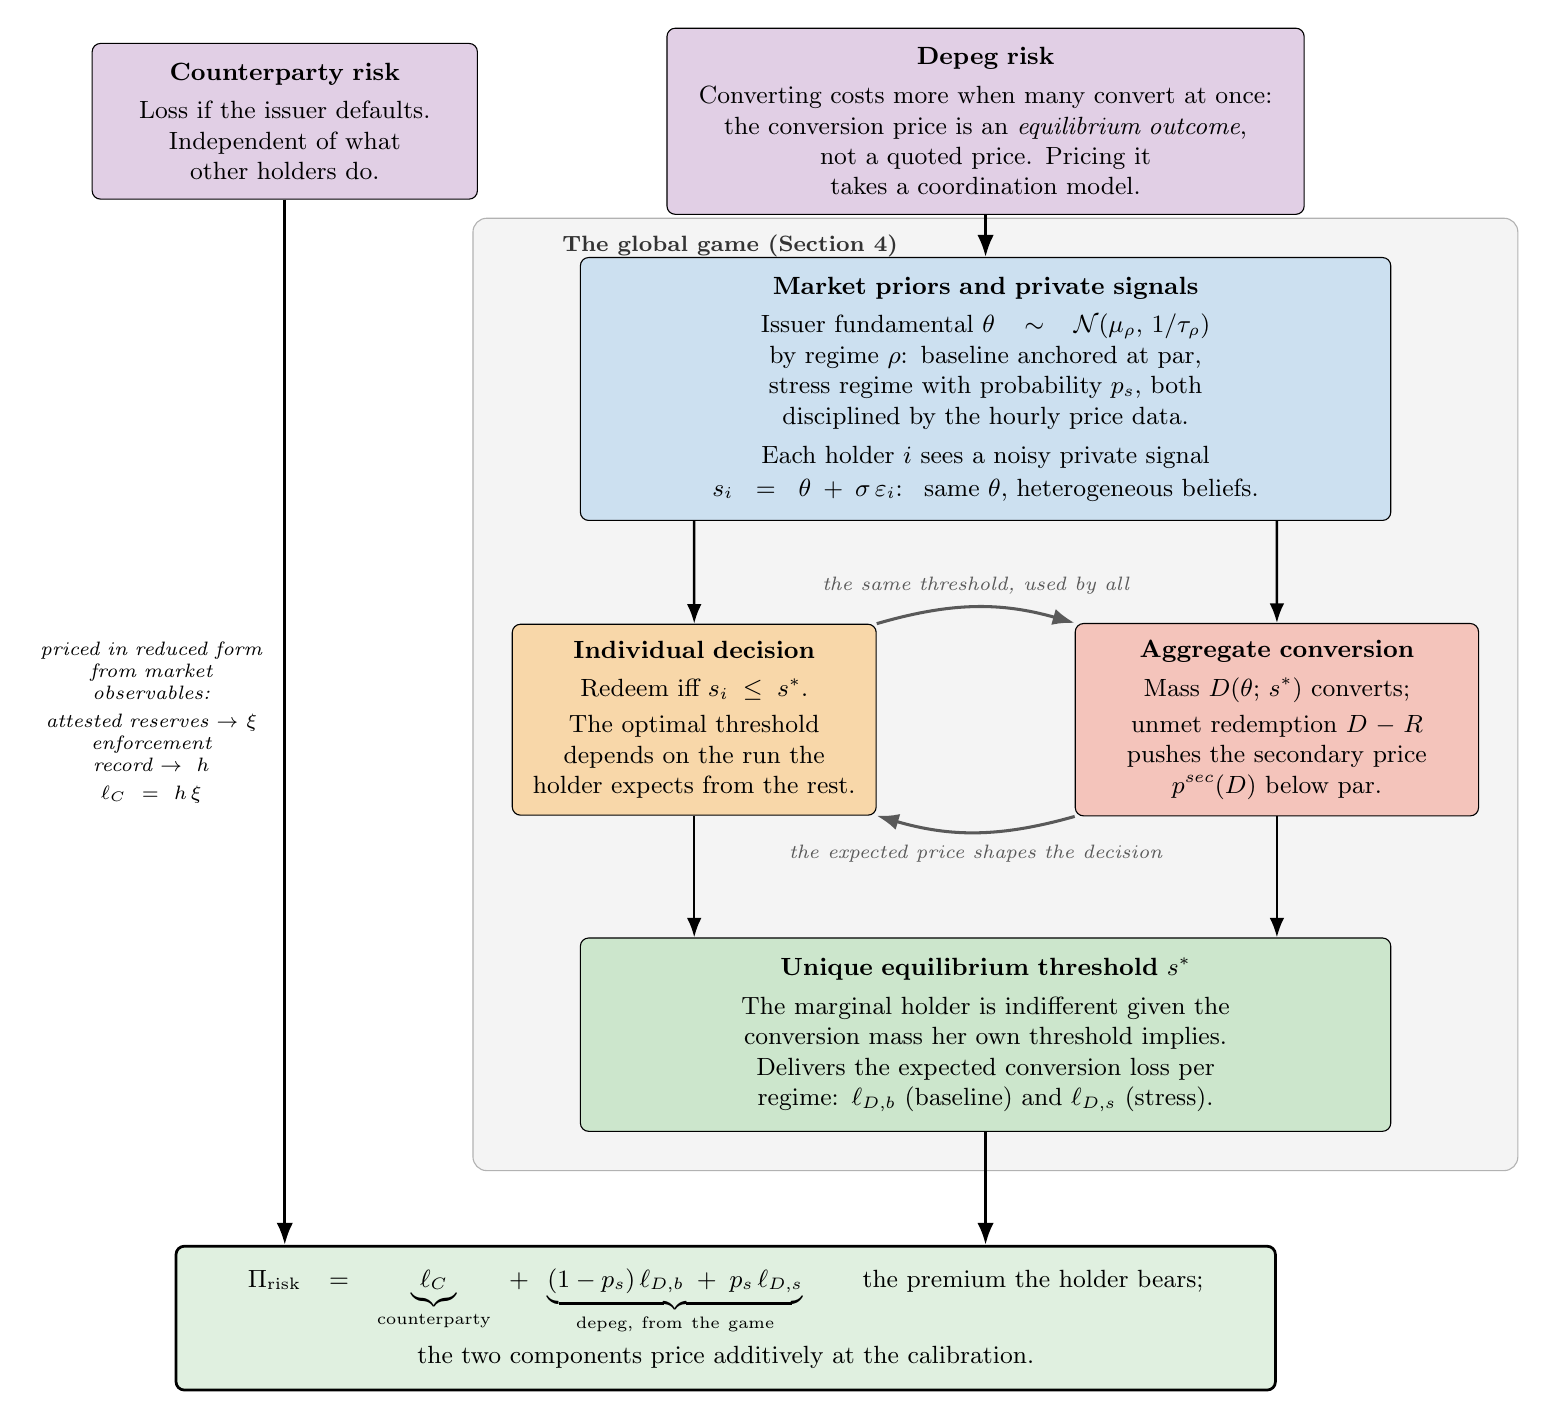
\begin{tikzpicture}[
  font=\small,
  every node/.style={align=center},
  riskbox/.style={rectangle, rounded corners=3pt, draw, fill=riskpurple,
                  inner sep=7pt},
  infobox/.style={rectangle, rounded corners=3pt, draw, fill=infoblue,
                  inner sep=7pt},
  bestbox/.style={rectangle, rounded corners=3pt, draw, fill=stratorange,
                  inner sep=6pt},
  aggbox/.style={rectangle, rounded corners=3pt, draw, fill=aggred,
                 inner sep=6pt},
  fpbox/.style={rectangle, rounded corners=3pt, draw, fill=eqgreen,
                inner sep=7pt},
  prembox/.style={rectangle, rounded corners=3pt, draw=black, line width=1pt,
                  fill=eqgreen!60, inner sep=8pt},
  looplab/.style={font=\scriptsize\itshape, fill=gamegray, inner sep=2pt},
  routelab/.style={font=\scriptsize\itshape, fill=white, inner sep=2pt},
  >=Latex
]

% ---- Top layer: the two risks ----------------------------------------------
\node[riskbox, text width=4.4cm] (cprisk) at (-6.0, 10.2) {%
  \textbf{Counterparty risk}\\[3pt]
  Loss if the issuer defaults.\\
  Independent of what\\
  other holders do.
};

\node[riskbox, text width=7.6cm] (dprisk) at (2.9, 10.2) {%
  \textbf{Depeg risk}\\[3pt]
  Converting costs more when many convert at once:\\
  the conversion price is an \emph{equilibrium outcome},\\
  not a quoted price. Pricing it takes a coordination model.
};

% Label of the game frame, outside its top-left corner
\node[font=\footnotesize\bfseries, anchor=south west, gray!40!black]
  at (-2.6, 8.35) {The global game (Section 4)};

% ---- Information layer: where the market priors enter ----------------------
\node[infobox, text width=9.8cm] (info) at (2.9, 6.8) {%
  \textbf{Market priors and private signals}\\[3pt]
  Issuer fundamental $\theta \sim \mathcal{N}(\mu_\rho,\,1/\tau_\rho)$ by regime $\rho$:
  baseline anchored at par,\\
  stress regime with probability $p_s$, both disciplined by the hourly price data.\\[3pt]
  Each holder $i$ sees a noisy private signal\\[1pt]
  $s_i = \theta + \sigma\,\varepsilon_i$: \ same $\theta$, heterogeneous beliefs.
};

% ---- Strategic loop ---------------------------------------------------------
\node[bestbox, text width=4.2cm] (best) at (-0.8, 2.6) {%
  \textbf{Individual decision}\\[3pt]
  Redeem iff $s_i \le s^{*}$.\\[2pt]
  The optimal threshold\\
  depends on the run the\\
  holder expects from the rest.
};

\node[aggbox, text width=4.7cm] (agg) at (6.6, 2.6) {%
  \textbf{Aggregate conversion}\\[3pt]
  Mass $D(\theta;\,s^{*})$ converts;\\[2pt]
  unmet redemption $D-R$\\
  pushes the secondary price\\
  $p^{sec}(D)$ below par.
};

\draw[->, line width=1.1pt, gray!70!black]
  (best.north east) to[bend left=16]
  node[looplab, midway, above=2pt] {the same threshold, used by all}
  (agg.north west);

\draw[->, line width=1.1pt, gray!70!black]
  (agg.south west) to[bend left=16]
  node[looplab, midway, below=2pt] {the expected price shapes the decision}
  (best.south east);

% ---- Fixed point ------------------------------------------------------------
\node[fpbox, text width=9.8cm] (fp) at (2.9, -1.4) {%
  \textbf{Unique equilibrium threshold $s^{*}$}\\[3pt]
  The marginal holder is indifferent given the conversion mass her own threshold implies.\\
  Delivers the expected conversion loss per regime: $\ell_{D,b}$ (baseline) and $\ell_{D,s}$ (stress).
};

% Game frame drawn behind
\begin{scope}[on background layer]
\node[rectangle, rounded corners=5pt, draw=gray!60, fill=gamegray,
      fit=(info)(best)(agg)(fp), inner sep=14pt] (gameframe) {};
\end{scope}

% ---- Bottom layer: the premium ----------------------------------------------
\node[prembox, text width=13.4cm] (prem) at (-0.4, -5.0) {%
  $\Pi_{\text{risk}} \;=\; \underbrace{\ell_C}_{\text{counterparty}}
  \;+\; \underbrace{(1-p_s)\,\ell_{D,b} \;+\; p_s\,\ell_{D,s}}_{\text{depeg, from the game}}$
  \qquad the premium the holder bears;\\[3pt]
  the two components price additively at the calibration.
};

% ---- Routes -------------------------------------------------------------------
% Left route: counterparty priced in reduced form, bypassing the game
\draw[->, line width=1.1pt]
  (cprisk.south) -- node[routelab, pos=0.5, left=3pt, text width=3.0cm]
  {priced in reduced form\\ from market observables:\\[2pt]
   attested reserves $\to \xi$\\
   enforcement record $\to h$\\[2pt]
   $\ell_C = h\,\xi$}
  (cprisk.south |- prem.north);

% Right route: depeg priced through the game
\draw[->, line width=1.1pt] (dprisk.south) -- (info.north);
\draw[->, line width=0.9pt] ([xshift=-3.7cm] info.south) -- (best.north);
\draw[->, line width=0.9pt] ([xshift=3.7cm] info.south) -- (agg.north);
\draw[->, line width=0.9pt] (best.south) -- (best.south |- fp.north);
\draw[->, line width=0.9pt] (agg.south)  -- (agg.south  |- fp.north);
\draw[->, line width=1.1pt] (fp.south) -- (fp.south |- prem.north);

\end{tikzpicture}

\end{document}
